\documentclass[letterpaper]{article}

\usepackage{amsmath}
\usepackage{amssymb}
\usepackage{amsthm}
\usepackage{booktabs}
\usepackage{commath}
\usepackage{lmodern}
\usepackage{microtype}
\usepackage{hyperref}
\usepackage{graphicx}

\author{Philip Pham}
\title{Scaling Gaussian Processes}
\date{\today}
\usepackage{natbib}
\bibliographystyle{unsrtnat}

\begin{document}
\maketitle

\section*{Introduction}

A Gaussian process is a collection of random variables finite number of which
have a joint Gaussian distribution \citep{gpbook}. Thus, a Gaussian process over an input space
$\mathcal{X}$ can be defined by

\begin{align*}
  m(\mathbf{x})
  &= \mathbb{E}\left[f\left(\mathbf{x}\right)\right] \\
  k(\mathbf{x}, \mathbf{x}^\prime)
  &= \mathbb{E}\left[
    (f(\mathbf{x}) - m(\mathbf{x}))
    (f(\mathbf{x}^\prime) - m(\mathbf{x}^\prime))
    \right]
\end{align*}
for any $\mathbf{x}, \mathbf{x}^\prime \in \mathcal{X}$. More concisely, we can
write
\begin{equation}
  f\left(\mathbf{x}\right)
  \sim
  \mathcal{GP}\left(
    m\left(\mathbf{x}\right),
    k\left(\mathbf{x},\mathbf{x}^\prime\right)
  \right).
\end{equation}
A Gaussian process is determined by its mean function and kernel function. The
kernel function can intuitively be thought as a similarity function between two
examples.

\section*{Regression}

Typically, we want to estimate $f$. Denote the estimate as $\hat{f}$.

We can view this from a Bayesian perspective. Let $K(X, X^\prime)$ be the kernel
matrix for observations between $X$ and $X^\prime$. Suppose we want predictions
for $X_*$. Our prior could be
$f(X_*) \sim \mathcal{N}\left(\mathbf{0}, K(X_*, X_*\right)$. After observing
$f\left(X\right)$, we have the posterior,
\begin{align*}
  f(X_*) &\mid X_*, X, f(X) \sim \\
  &\mathcal{N}\left(
  K(X_*, X)K(X,X)^{-1}f(X),
  K(X_*,X_*) - K(X_*,X)K(X,X)^{-1}K(X,X_*)
  \right).
\end{align*}
by properties of the multivariate Gaussian distribution \citep{gpbook}.

Another way of expressing this is with reproducing kernel Hilbert spaces
(RKHS). If $\mathbf{x}_*$ is a single test point, we have that
\begin{align*}
  f\left(\mathbf{x}_*\right)
  &= \sum_{i=1}^n\alpha_ik(x_i, x_*),
\end{align*}
by the representer theorem. Here, $\alpha = K(X,X)^{-1}\mathbf{y}$, where
$\mathbf{y} = f(X)$ is observed.

\section*{Classification}

Regression extends to classification by modeling the latent variables (logits)
as a Gaussian process. The class probabilities are obtained by taking a softmax
over these latent variables \citep{gpbook}.

In this case, we observe $(X, \mathbf{y})$, but we don't oberve the latent
variables $f(X)$, so the previous equations are no longer possible to
apply. Instead we have a integeral to estimate $f_*$:
\begin{equation*}
  p\left(f_* \mid X, \mathbf{y}, x_*\right) =
    \int p(f_*\mid X, \mathbf{y}, x_*, f) p\left(f \mid X, \mathbf{y}\right) df.
  \end{equation*}

  If we choose $p$ as the categorical distribution and use the Laplace
  approximation, we our maximizing the unnormalized probability,
  \begin{equation}
    \Psi(f) = -\frac{1}{2}f^\intercal K^{-1} f + y^\intercal f
     - \sum_{i=1}^n\log\left(\sum_{c=1}^C \exp f_i^c\right),
   \end{equation}
   where we have $C$ classes. After finding $f$ by maximizing this equation, we
   can apply the same equations as in the regression case.

   For the variance, we use the law of total variance:
   \begin{equation}
     \operatorname{var}(f_* \mid X, \mathbf{y}, x_*) =
     \operatorname{var}(f_* \mid X, x_*, f)
     +
     \mathbb{E}_{q(f \mid X, y)}\left[
       \operatorname{var}(f_* \mid X, x_*, f)
     \right].
   \end{equation}
   The first term is the same as regression. The second term we can use the
   Gaussian approxmiation.

   \section*{Experiments}

   I decided to run classification experiments on MNIST
   \citep{lecun2010mnist}. The training set has 60,000 examples. Unfortunately
   this is prohibitively expensive since we have to invert $K$, which is
   $O(n^3)$. I used a Gaussian kernel and a bandwidth of 64, which was bound by
   evaluating on a hold-out set of examples.

   \begin{figure}
     \centering
     
\includegraphics[width=0.15\textwidth]{2_image.pdf}
     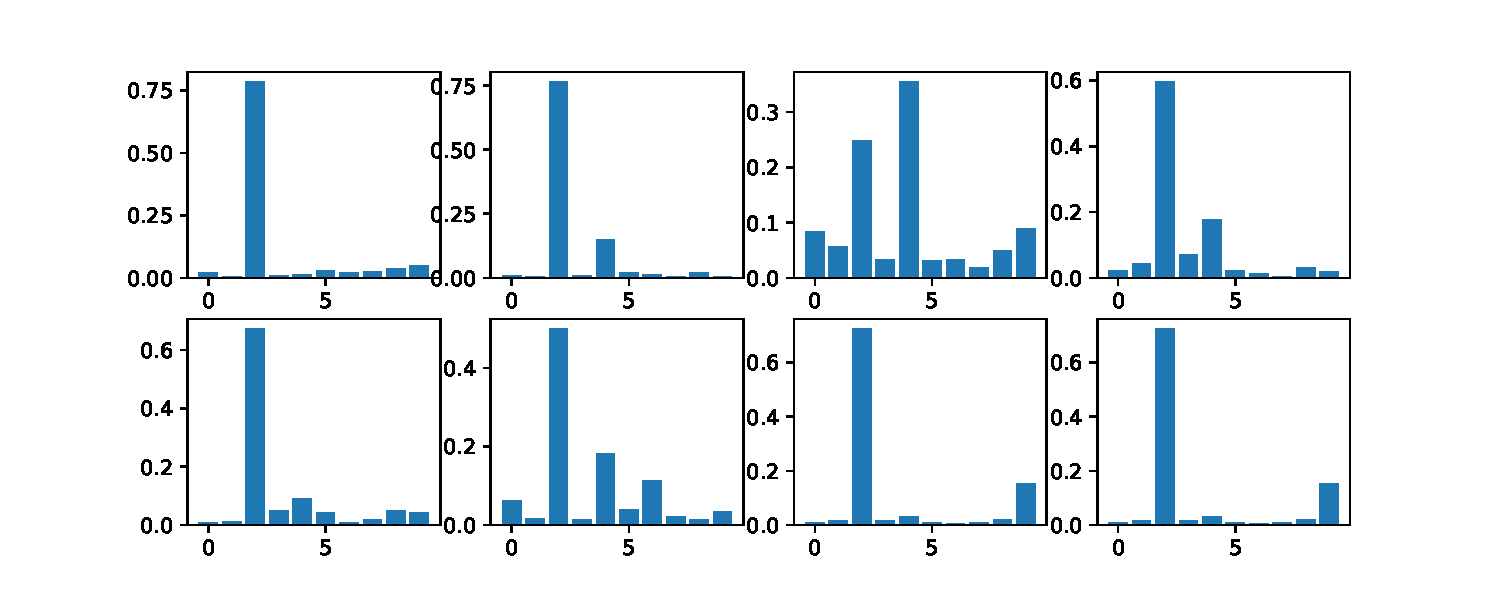
\includegraphics[width=0.84\textwidth]{2_distribution.pdf}
     \caption{Samples of $\operatorname{softmax}(f_*)$ for a correctly predicted
       example. You can see sharp peak at 2 for most of the samples.}
     \label{fig:2}
   \end{figure}

   \begin{figure}
     \centering
     
\includegraphics[width=0.15\textwidth]{8_image.pdf}
     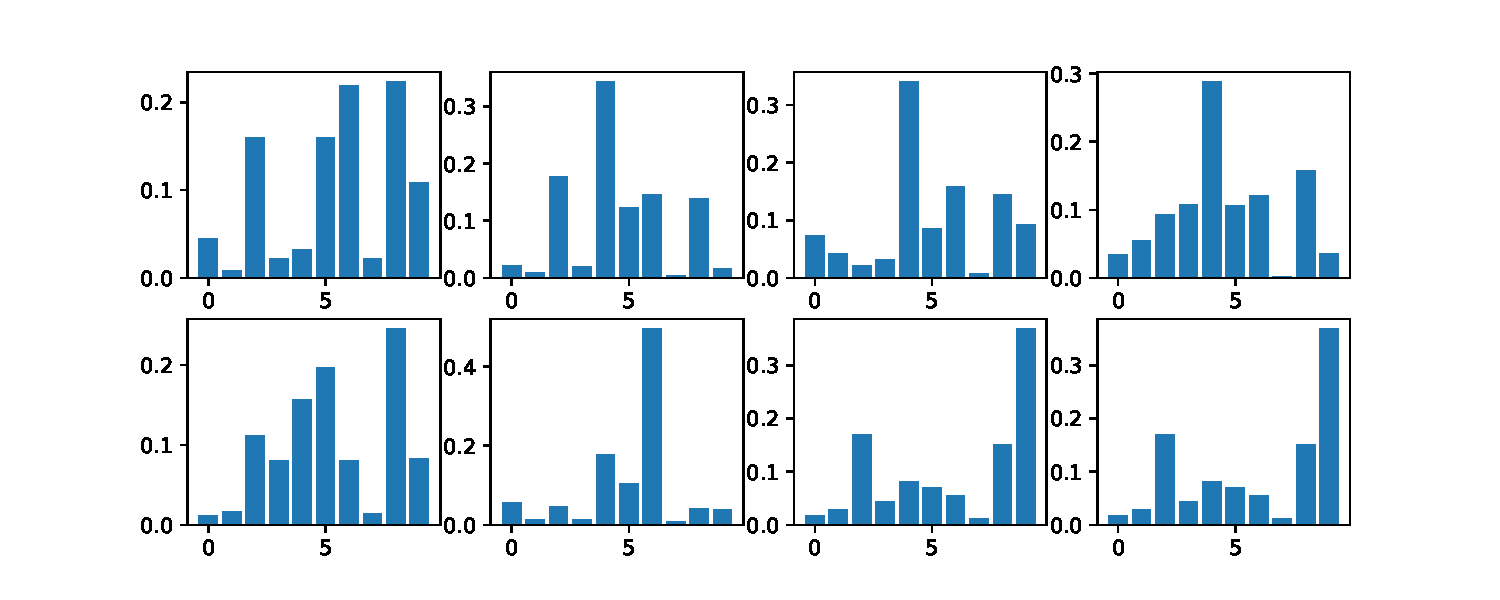
\includegraphics[width=0.84\textwidth]{8_distribution.pdf}
     \caption{Samples of $\operatorname{softmax}(f_*)$ for an incorrectly
       predicted example. The samples here are much more random.}
     \label{fig:8}
   \end{figure}

   One nice property of Gaussian processes is that you can get real uncertainty
   estimates. See Figures \ref{fig:2} and \ref{fig:8}. In the first Figure, the
   model is quite certain about the 2 prediction: in almost every sample, there
   is a sharp peak at 2. For the 8, the model predicts 6, but is uncertain, for
   only one of the samples has its highest peak at 6.
   
   \subsection*{Sub-sampling}

   One way to make the run feasible is to throw away some training data.

   \begin{table}
     \centering
     \begin{tabular}{lr}
       \toprule
       Fraction of data & Test set accuracy \\
       \midrule
       0.01 & 0.86370003 \\
       0.02 & 0.89220005 \\
       0.04 & 0.919 \\
       0.08 & 0.9355 \\
       0.16 & 0.9498001 \\
       0.32 & 0.96220005 \\
       \bottomrule
     \end{tabular}
     \caption{Test set accuracy by degree of sampling.}
     \label{tab:test_acc}
   \end{table}

   See Table \ref{tab:test_acc} for the results of this experiment. Clearly more
   data helps. Any attempts to scale further were met with out of memory errors.

   Code for these experiments can be found in
   \href{https://github.com/ppham27/stat527/blob/master/project/mnist.ipynb}{\texttt{mnist.ipynb}}.

   \subsection*{Reduced Rank}

   I would have liked to try the
   \href{https://en.wikipedia.org/wiki/Low-rank_matrix_approximations}{Nyostrom
     Approximation}.

   \bibliography{references}
\end{document}
